% Forrás: Fleiner Tamás gyakorlat

\documentclass[tikz]{standalone}
\usepackage{tikz}
\usetikzlibrary{positioning, graphs}
\usetikzlibrary{graphs.standard}
\begin{document}
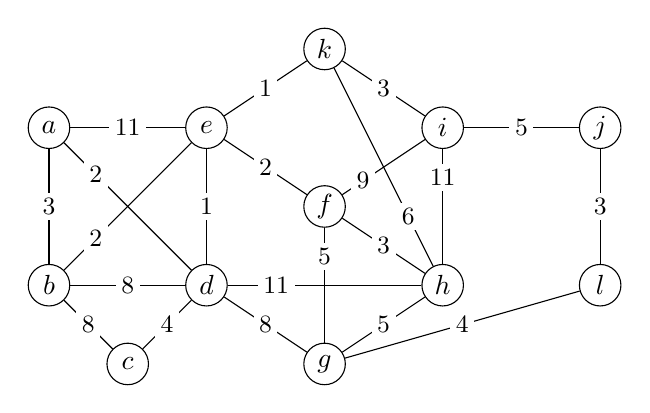
\begin{tikzpicture}
		[vertex/.style={draw,circle,inner sep = 0mm, minimum size = 15},
         edgelabel/.style = {fill = white, inner sep = 2, font=\small}]

        \node[vertex] (a) at (0.0,  0.0) {$a$};
        \node[vertex] (b) at (0.0, -2.0) {$b$};
        \node[vertex] (c) at (1.0, -3.0) {$c$};
        \node[vertex] (d) at (2.0, -2.0) {$d$};
        \node[vertex] (e) at (2.0,  0.0) {$e$};
        \node[vertex] (f) at (3.5, -1.0) {$f$};
        \node[vertex] (g) at (3.5, -3.0) {$g$};
        \node[vertex] (h) at (5.0, -2.0) {$h$};
        \node[vertex] (i) at (5.0,  0.0) {$i$};
        \node[vertex] (j) at (7.0,  0.0) {$j$};
        \node[vertex] (k) at (3.5,  1.0) {$k$};
        \node[vertex] (l) at (7.0, -2.0) {$l$};

        \draw[-] (a) to node[edgelabel] {$11$} (e);
        \draw[-] (a) to node[edgelabel] {$3$} (b);
        \draw[-] (a) to node[edgelabel, near start] {$2$} (d);
        \draw[-] (b) to node[edgelabel] {$8$} (c);
        \draw[-] (b) to node[edgelabel] {$8$} (d);
        \draw[-] (b) to node[edgelabel, near start] {$2$} (e);
        \draw[-] (c) to node[edgelabel] {$4$} (d);
        \draw[-] (d) to node[edgelabel] {$1$} (e);
        \draw[-] (d) to node[edgelabel] {$8$} (g);
        \draw[-] (d) to node[edgelabel, near start] {$11$} (h);
        \draw[-] (e) to node[edgelabel] {$2$} (f);
        \draw[-] (e) to node[edgelabel] {$1$} (k);
        \draw[-] (f) to node[edgelabel, near start] {$5$} (g);
        \draw[-] (f) to node[edgelabel] {$3$} (h);
        \draw[-] (f) to node[edgelabel, near start] {$9$} (i);
        \draw[-] (g) to node[edgelabel] {$5$} (h);
        \draw[-] (g) to node[edgelabel] {$4$} (l);
        \draw[-] (h) to node[edgelabel, near end] {$11$} (i);
        \draw[-] (h) to node[edgelabel, near start] {$6$} (k);
        \draw[-] (i) to node[edgelabel] {$5$} (j);
        \draw[-] (i) to node[edgelabel] {$3$} (k);
        \draw[-] (j) to node[edgelabel] {$3$} (l);
		
\end{tikzpicture}
\end{document}